\documentclass{article}
\usepackage{graphicx}
\usepackage{tikz}
\begin{document}

\begin{center}

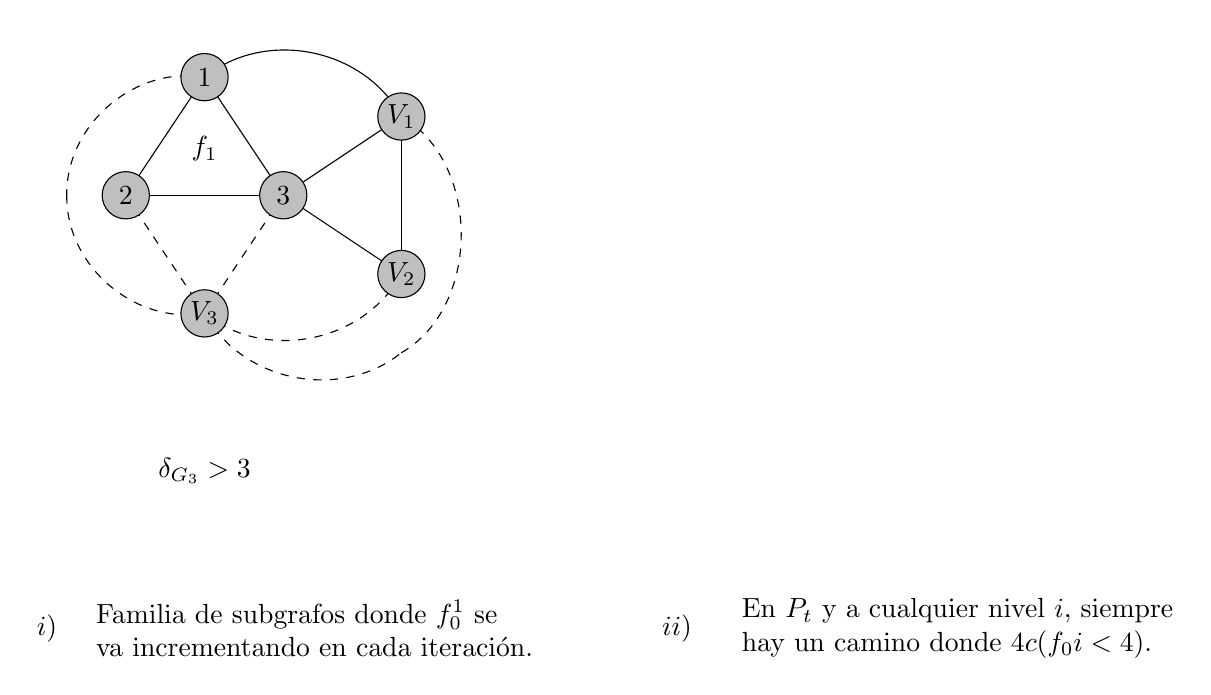
\begin{tikzpicture}
  \draw (4,14) -- (3,12.5);
  \draw (3,12.5) -- (5,12.5);
  \draw (5,12.5) -- (4,14);
  \draw[dashed] (3,12.5) -- (4,11);
  \draw[dashed] (5,12.5) -- (4,11);
  \draw (5,12.5) -- (6.5,13.5);
  \draw (6.5,13.5) -- (6.5,11.5);
  \draw (6.5,11.5) -- (5,12.5);
  \draw (4,14) to[bend left=50] (6.5,13.5);
  \draw[dashed] (4,11) to[bend right=50] (6.5,11.5);
  \draw[dashed] (4,11) to[bend right=50] (6.5,10.5);
  \draw[dashed] (6.5,10.5) to[bend right=60] (6.5,13.5);
  \draw[dashed] (4,14) to[bend right=50] (2.25,12.5);
  \draw[dashed] (2.25,12.5) to[bend right=50] (4,11);

  \filldraw[fill=lightgray] (4,14) circle (0.3) node{1} node[below=18pt]{$f_{1}$};
  \filldraw[fill=lightgray] (3,12.5) circle (0.3) node{2};
  \filldraw[fill=lightgray] (5,12.5) circle (0.3) node{3};
  \filldraw[fill=lightgray] (4,11) circle (0.3) node{$V_{3}$};
  \filldraw[fill=lightgray] (6.5,13.5) circle (0.3) node{$V_{1}$};
  \filldraw[fill=lightgray] (6.5,11.5) circle (0.3) node{$V_{2}$};

  \node at (4,9) {$\delta_{G_3} > 3$}; 
  \node at (2,7) {$i$)};
  \node[anchor=west, align=left] at (2.5,7)
  {Familia de subgrafos donde $f_{0}^1$ se\\
  va incrementando en cada iteración.};
  \node at (10,7) {$ii$)};
  \node[anchor=west, align=left] at (10.7,7)
  {En $P_{t}$ y a cualquier nivel $i$, siempre\\
  hay un camino donde $4c(f_{0}i<4)$.};
  
\end{tikzpicture}

\end{center}
\end{document}
